\documentclass[a4paper,12pt]{article}
\usepackage[top = 2.5cm, bottom = 2.5cm, left = 2.5cm, right = 2.5cm]{geometry}
% Unfortunately, LaTeX has a hard time interpreting German Umlaute. The following two lines and packages should help. If it doesn't work for you please let me know.
\usepackage[T1]{fontenc}
\usepackage[utf8]{inputenc}
% The following two packages - multirow and booktabs - are needed to create nice looking tables.
\usepackage{multirow} % Multirow is for tables with multiple rows within one cell.
\usepackage{booktabs} % For even nicer tables.
% As we usually want to include some plots (.pdf files) we need a package for that.
\usepackage{graphicx}
% The default setting of LaTeX is to indent new paragraphs. This is useful for articles. But not really nice for homework problem sets. The following command sets the indent to 0.
\usepackage[spanish]{babel}
\usepackage{setspace}
\setlength{\parindent}{0in}
% Package to place figures where you want them.
\usepackage{float}
% The fancyhdr package let's us create nice headers.
\usepackage{fancyhdr}
\usepackage{amsmath}
\usepackage{amssymb}
\usepackage{amsthm}
\usepackage{natbib}
\usepackage{graphicx}
\usepackage{subcaption}
\usepackage{booktabs}
\usepackage{etoolbox}
\usepackage{apalike}
\usepackage{minibox}
\AtBeginEnvironment{align}{\setcounter{equation}{0}}

\pagestyle{fancy}

\fancyhf{}

\lhead{\footnotesize HT 2}
\rhead{\footnotesize  Rompich}
\cfoot{\footnotesize \thepage}

\begin{document}
    \thispagestyle{empty} % This command disables the header on the first page.

    \begin{tabular}{p{15.5cm}} % This is a simple tabular environment to align your text nicely
    \begin{tabbing}
    Universidad del Valle de Guatemala \\
    Departamento de Matemática\\
    Licenciatura en Matemática Aplicada
    \\8 de marzo de 2021  \\
    Rudik Roberto Rompich   - Carné: 19857\\
    \end{tabbing}
    Análisis de Variable Real 1 - Dorval Carías \\
    \hline % \hline produces horizontal lines.
    \\
    \end{tabular} % Our tabular environment ends here.
    \vspace*{0.3cm} % Now we want to add some vertical space in between the line and our title.
    \begin{center} % Everything within the center environment is centered.
    {\Large \bf HT 2
} % <---- Don't forget to put in the right number
        \vspace{2mm}
    \end{center}
    \vspace{0.4cm}
\section{Ejercicios}
\textit{Definiciones y Teoremas:} (Se considerarán las definiciones y teoremas del libro de \citeauthor{bartle2000introduction}.
\newline\newline
\minibox[frame]{ Definición 1. Se dice que una secuencia $X= (x_n)$ en $\mathbf{R}$ converge a un $x\in\mathbf{R}$, si para cada $\epsilon<0$\\ existe un número natural $K(\epsilon)$ tales que para todos $n\geq K(\epsilon)$, los términos de $x_n$ satisfacen\\ $|x_n-x|<\epsilon$}
\newline
\newline
\minibox[frame]{ Definición 2. Una $X=(x_n)$ de números reales se dice que es una secuecia de Cauchy si para ca-\\da $\epsilon>0$ existe un número natural $H(\epsilon)$ tal que para todos los números naturales $n,m\geq H(\epsilon)$\\, los términos $x_n,x_m$ satisfacen $|x_n-x_m|<\epsilon$}
\newline
\newline
\minibox[frame]{Definición 3. Una secuencia $X=(x_n)$ de números reales se dice que es acotada si existe un núm\\ero real $M>0$ tal que $|x_n|\leq M$ para todo $n\in\mathbf{N}$.}
\newline
\newline
\minibox[frame]{Definición 4. Sea una secuencia $X=(x_n)$ de números reales. Se dice que es creciente si satisface\\
$x_1\leq x_2\leq...\leq x_n\leq x_{n+1}\leq ...$}
\newline
\newline
\minibox[frame]{Teorema 1. \textbf{Teorema de la convergencia monótona}. Una secuencia monótona de números\\ reales es convergente si y solo si es acotada. Es decir (en el caso de cota superior): Si $X=(x_n)$\\ es una secuencia acotada
creciente, entonces: $\lim(x_n)=sup\{x_n:n\in \mathbf{N}\}$}
\newline
\newline
\minibox[frame]{Teorema 2. Sea $X=(x_n:n\in\mathbf{N})$ una secuencia de números y sea $m\in\mathbf{N}$. Entonces la $m-$cola\\ $X_m=(X_{m+n}:n\in\mathbf{N}$ de $X$ converge si y solo si $X$ converge. En este caso, $\lim X_m=\lim X$.}
%---------------------------
\newpage
\subsection{Problema 1} Demuestre que una secuencia monótona creciente y acotada es de Cauchy.
\begin{proof}
\begin{align}
    \intertext{Por hipótesis, sabemos que existe una secuencia $(x_n)$ que es acotada y monótona creciente. Asumamos que $u=\lim(x_n)=\sup\{x_n:n\in\mathbf{N}\}$ (por Teorema 1),  $\epsilon>0$ y $H(\epsilon)\in \mathbf{N}$. Definamos $H(\epsilon)=H$; entonces, por definición de supremo, se debe cumplir: }
    u-\epsilon <x_H&\leq u
    \intertext{Por otra parte, supongamos $n\geq m\geq H$. Además, por hipótesis también sabemos que es una secuencia creciente, entonces tomamos la definición 4, en donde:}
    x_H \leq x_m&\leq x_n
    \intertext{Es decir, si combinamos (1) y (2), tenemos:}
    u-\epsilon <x_H&\leq x_m\leq x_n\leq u
    \intertext{Ahora bien, para determinar que es una secuencia de Cauchy, debemos comprobar que $|x_n-x_m|<\epsilon$ (según la definición 2). Notamos que se pueden sacar dos desigualdades de la expresión:}
    u-\epsilon &< x_m\leq u\\
    u-\epsilon &< x_n\leq u
    \intertext{Notamos que la desigualdad (4) la podemos expresar como: $ -1(u-\epsilon < x_m\leq u)\implies -u+\epsilon > -x_m\geq -u$. Entonces si sumamos los dos términos tenemos que:}
    -u&\leq -x_m< -u+\epsilon \\
    u-\epsilon &< x_n\leq u\\
    \implies (-u)+ (u-\epsilon) &< (x_n)+(-x_m)<(-u+\epsilon)+u\\
    \implies -\epsilon &< (x_n)+(-x_m)<\epsilon \\
    \implies |(x_n)+(-x_m)|&<\epsilon 
\end{align}
Por lo tanto, $(x_n)$ es una secuencia de Cauchy.
\end{proof}
%---------------------------
\subsection{Problema 2} Si $x_{n}=\sqrt{n},$ demuestre que $\left(x_{n}\right)$ satisface que $\left|x_{n+1}-x_{n}\right|=0,$ pero no es una sucesión de Cauchy.
%---------------------------
\begin{proof}
\begin{align}
\intertext{Consideremos $x_{n+1}=\sqrt{n+1}$, entonces la expresión:}
|x_{n+1}-x_n| &=|\sqrt{n+1}-\sqrt{n}|
\intertext{Considerando que es necesario encontrar $\lim(|\sqrt{n+1}-\sqrt{n}|)=0$. Se propone otra notación para tratar el problema. Primero, sabemos que $\left(\frac{\sqrt{n+1}+\sqrt{n}}{\sqrt{n+1}+\sqrt{n}}\right)=1$,por lo que se tiene:}
&= \left|\left(\sqrt{n+1}-\sqrt{n}\right)\cdot\left(\frac{\sqrt{n+1}+\sqrt{n}}{\sqrt{n+1}+\sqrt{n}}\right)\right|\\
&= \left|\frac{(n+1)+\sqrt{n}\sqrt{n+1}-\sqrt{n}\sqrt{n+1}-n}{\sqrt{n+1}+\sqrt{n}}\right|\\
&= \left| \frac{1}{\sqrt{n+1}+\sqrt{n}}\right|
\intertext{Es decir, que tenemos $\lim\left(|\sqrt{n+1}-\sqrt{n}\right|) = \lim\left(\left|  \frac{1}{\sqrt{n+1}+\sqrt{n}}\right|\right)=0$, para comprobarlo, usamos la definición 1, dado $\epsilon>0$ entonces $\exists N= \left(\frac{1}{2\epsilon}\right)^2$ tal que $n\geq \left(\frac{1}{2\epsilon}\right)^2$ y que satisface $|x_n-x|<\epsilon$:}
\left|\frac{1}{\sqrt{n+1}+\sqrt{n}}\right| &\leq \left|\frac{1}{\sqrt{n}+\sqrt{n}}\right| = \left|\frac{1}{2\sqrt{n}}\right|<\epsilon
\intertext{Despejando para $n$ y tomando en cuenta el caso positivo:}
n &= \left(\frac{1}{2\epsilon}\right)^2  
\intertext{Por lo tanto, sabemos que el límite de la secuencia es cero. Por otra parte, para comprobar que no es una secuencia de Cauchy, se propone un contraejemplo: $\frac{1}{2\sqrt{1}}=\frac{1}{2}<\epsilon, n=n, m=4n$, entonces se tiene: }
|x_m-x_n| &= |(\sqrt{4n})-(\sqrt{n})| = |2(\sqrt{n})-(\sqrt{n})| =|\sqrt{n}|
\end{align}
Entonces, sabemos que $\sqrt{n}$ siempre tiene que ser $\geq 1$. Por lo tanto, no cumple con la definición 2, que afirma que se debe satisfacer $|x_n-x_m|<\epsilon$. Entonces, no es una sucesión de Cauchy. 
\end{proof}
%---------------------------
\subsection{Problema 3} Si $x_{1}<x_{2}$ son números reales arbitrarios y $x_{n}=\frac{1}{2}\left(x_{n-2}+x_{n-1}\right)$ para $n>2,$ pruebe
que $\left(x_{n}\right)$ converge. Encuentre el límite.
\newline
%---------------------------
\minibox[frame]{La siguiente demostración, tomará como referencia el ejercicio resuelto en clase en donde\\ $x_1=1$ y $x_2=2$.}
%---------------------------
\begin{proof} 
Es necesario demostrar que $(x_n)$ converge, es decir, tenemos dos posibilidades:
\begin{enumerate}
    \item Si la serie es monótona se podría usar el \text{Teorema de Convergencia Monótona}. Propongamos $n=1$, entonces se tiene $x_3=\frac{1}{2}(x_1+x_2)<x_2$. Entonces, $(x_n)$ no es monótona y por lo tanto no se puede utilizar para demostrar convergencia.
    \item Si $(x_n)$ es una secuencia de Cauchy, entonces debe converger.  
\end{enumerate}
Procedemos a probar que $(x_n)$ es de Cauchy (basándonos en la definición 2). Primero, ya que los términos son generados por un promedio, es necesario encontrar una relación entre $|x_n-x_{n+1}|$:
\begin{align}
    |x_n-x_{n+1}|&=\left|x_n-\left( \frac{x_n+x_{n-1}}{2}\right)\right|= \frac{1}{2}|x_n-x_{n-1}|\\
    &=\frac{1}{2^2}|x_{n-1}-x_{n-2}| = \frac{1}{2^3}|x_{n-2}-x_{n-3}|=...=\frac{1}{2^{n-1}}|x_2-x_1|
    \intertext{En general, supongamos que $m>n$, entonces:}
    |x_n-x_m|&= |(x_n-x_{n+1})+(x_{n+1}-x_{n+2})+...+(x_{m-1}-x_m)|\\
             &\leq |x_n-x_{n+1}|+|x_{n+1}-x_{x+2}|+...+|x_{m-1}-x_m|\\
             &= \left[\frac{1}{2^{n-1}}+\frac{1}{2^n}+\frac{1}{2^{m+1}}+...+\frac{1}{2^{m-2}}\right]|x_2-x_1|\\
             &= \left[\frac{1}{2^{n-1}}\left( 1+\frac{1}{2}+\frac{1}{2^2}+...+\frac{1}{2^{n-m-1}}\right)\right]|x_2-x_1|\\
             &= \left[\frac{1}{2^{n-1}}\sum_{n=0}^{\infty}\left(\frac{1}{2}\right)^n\right]|x_2-x_1|\\
             &= \left[\frac{1}{2^{n-1}}\left(\frac{1}{1-\left(\frac{1}{2}\right)}\right)\right]|x_2-x_1|\\
             &= \left[\frac{2}{2^{n-1}}\right]|x_2-x_1|\\
             &= \left[\frac{1}{2^{n-2}}\right]|x_2-x_1|
    \intertext{Es decir, que $|x_n-x_m|\leq [2^{2-n}]|x_2-x_1|$. Entonces, dado $\epsilon>0\exists H=\log_2\left(\frac{4|x_2-x_1|}{\epsilon} \right)\in \mathbf{Z^+}\ni$ si $n,m>H\implies |x_n-x_m|<\epsilon$ tal que:}
    [2^{2-n}]|x_2-x_1| < \epsilon&\implies[2^2 2^{-n}] < \frac{\epsilon}{|x_2-x_1|}\implies \frac{1}{2^n}< \frac{\epsilon}{4|x_2-x_1|} \\
    &\implies 2^n >\frac{4|x_2-x_1|}{\epsilon}\implies \log_2(2^n)>\log_2\left(\frac{4|x_2-x_1|}{\epsilon} \right)\\
    &\implies n>\log_2\left(\frac{4|x_2-x_1|}{\epsilon} \right)
    \intertext{Por lo tanto, es una sucesión de Cauchy y por criterio de Cauchy, la sucesión debe converger. Como $(x_n)$ converge,  procedemos a encontrar su límite por la subsecuencia de números impares $x_{2n-1}$, es decir:}
    x_{2n-1} &= x_1+\frac{|x_2-x_1|}{2}+ \frac{|x_2-x_1|}{2^3}+\frac{|x_2-x_1|}{2^5}+...+\frac{|x_2-x_1|}{2^{2n-1}}
    \intertext{Como $x_2>x_1$, entonces podemos quitar el valor absoluto. Se procede con lo siguiente:}
    \lim(x_n) &= x_1+\frac{2}{3}(x_2-x_1)\\
              &= x_1 +\frac{2}{3}x_2-\frac{2}{3}x_1\\
              &= \frac{1}{3}x_1+\frac{2}{3}x_2
    \end{align}

\end{proof}
%---------------------------
\subsection{Problema 4} Sea $\alpha \in(0,2)$. Considere la sucesión definida por:
$$
x_{n+1}=\alpha x_{n}+(1-\alpha) x_{n-1}, \forall n \geq 1
$$
Encuentre el límite de la sucesión en términos de $\alpha, x_{0}, x_{1}$.
%---------------------------
\begin{proof}
Según las condiciones del problema, es necesario encontrar el límite de la sucesión en términos de $\alpha,x_0,x_1$. Se propone, el método para sucesiones de recurrencia de segundo orden, es decir: 
\begin{align}
\intertext{Tenemos:}
    x_{n+1}&=\alpha x_{n}+(1-\alpha) x_{n-1}
\intertext{Si asignamos arbitrariamente $x^2=x_{x+1}, x= x_n$ y $1=x_{n-1}$:}
    x^2&=\alpha x+(1-\alpha)\\
    0  &= x^2-\alpha x+(a-1)\\
\intertext{Aplicamos la fórmula de Vieta y encontramos que $x_1=(\alpha-1)$ y $x_2=1$, entonces se tiene:}
    x_{n+1}&= C_1(\alpha-1)^n+C_2(1)^n
\intertext{Será necesario encontrar las constantes $C_1$ y $C_2$. Por hipótesis, sabemos que tiene que estar en términos de $x_0,x_1,\alpha$ y $n\geq 1$.}
\intertext{Para $n=1$:}
        x_{1+1}&= C_1(\alpha-1)^1+C_2(1)^1\\
\intertext{Para $n=2$:}
        x_{2+1}&= C_1(\alpha-1)^2+C_2(1)^2\\
\intertext{Entonces tenemos el sistema de ecuaciones:}
&\begin{cases}
C_1(\alpha-1)^1+C_2=x_2\\
C_1(\alpha-1)^2+C_2=x_3\\
\end{cases}
\intertext{Consideremos también, que $x_2$ y $x_3$, tienen una igualdad con la expresión original:}
x_2 &= \alpha x_1+(1-\alpha)x_0\\
x_3 &= \alpha x_2+(1-\alpha)x_1\\
    &= \alpha [\alpha x_1+(1-\alpha)x_0]+(1-\alpha)x_1\\
    &= \alpha^2x_1+\alpha(1-\alpha)x_0+(1-\alpha)x_1\\
    &= (\alpha^2-\alpha+1)x_1+(\alpha-\alpha^2)x_0
\intertext{Entonces, aplicando una substitución a la segunda ecuación de (7):}
    C_1&= \frac{x_2-C_2}{(\alpha-1)}\\
    &\implies \left(\frac{x_2-C_2}{(\alpha-1)} \right)(\alpha-1)^2+C_2=x_3\\
    &\implies (x_2-C_2)(\alpha-1)+C_2=x_3\\
    &\implies \alpha x_2-x_2-\alpha C_2+2C_2=x_3\\
    &\implies (2-\alpha)C_2+(\alpha - 1)x_2=x_3\\
    C_2&= \frac{x_3-(\alpha-1)x_2}{2-\alpha}
    \intertext{Ahora bien, se substituye $C_2$ y $C_3$ con los valores de encontrados en (8) y (12): }
    C_2 &= \frac{(\alpha^2-\alpha+1)x_1+(\alpha-\alpha^2)x_0-(\alpha-1)[\alpha x_1+(1-\alpha)x_0]}{2-\alpha}\\
     &= \frac{(\alpha^2-\alpha+1)x_1+(\alpha-\alpha^2)x_0-(\alpha^2-\alpha)x_1+(1-\alpha)^2x_0}{2-\alpha}\\
     &= \frac{[(\alpha^2-\alpha+1)-(\alpha^2-\alpha)]x_1+[(\alpha-\alpha^2)+(1-\alpha)^2]x_0}{2-\alpha}\\
    &= \frac{x_1+[(\alpha-\alpha^2)+(1-2\alpha+\alpha^2)]x_0}{2-\alpha}\\
     &= \frac{x_1+(1-\alpha)x_0}{2-\alpha}\\
    \implies C_1 &= \frac{x_2-C_2}{\alpha-1}=\frac{[\alpha x_1+(1-\alpha)x_0]-\left(\frac{x_1+(1-\alpha)x_0}{2-\alpha}\right)}{\alpha-1}\\
    &= \frac{\frac{(\alpha x_1+(1-\alpha)x_0)(2-\alpha)-(x_1+(1-\alpha)x_0)}{2-\alpha}}{\alpha-1} = \frac{\frac{-(\alpha-1)^2x_1}{2-\alpha}}{\alpha-1}\\
    &= \frac{-(\alpha-1)x_1}{2-\alpha} =\frac{(1-\alpha)x_1}{2-\alpha}
    \intertext{Es decir que tenemos, substituyendo en la ecuación (4):}
    X_{n+1} &= C_1(\alpha-1)^n+C_2(1)^n\\
            &= \frac{(1-\alpha)x_1}{2-\alpha}(\alpha-1)^n+\frac{x_1+(1-\alpha)x_0}{2-\alpha}(1)^n\\
            &= \frac{(1-\alpha)x_1(\alpha-1)^n+(x_1+(1-\alpha)x_0)(1)^n}{2-a}\\
    \intertext{Se puede asumir que $(1)^n =1$ en todos los casos.}
            &= \frac{(1-\alpha)x_1(\alpha-1)^n+(x_1+(1-\alpha)x_0)}{2-a}\\
            &= \frac{-(\alpha-1)x_1(\alpha-1)^n+(x_1+(1-\alpha)x_0)}{2-a}\\
            &= \frac{-x_1(\alpha-1)^{n+1}+(x_1+(1-\alpha)x_0)}{2-a}\\
            &= \frac{-x_1(\alpha-1)^{n+1}+x_1+(1-\alpha)x_0}{2-a}\\
            &= \frac{[1-(\alpha-1)^{n+1}]x_1+(1-\alpha)x_0}{2-\alpha}
    \intertext{Entonces, la convergencia de la serie dependerá de la siguiente expresión, en donde $\alpha\in (0,2):$}
    \lim(x_n) &=  \frac{[1-(\alpha-1)^{n+1}]x_1+(1-\alpha)x_0}{2-\alpha}
    \end{align}

\end{proof}
%---------------------------
\subsection{Problema 5} Sea $a$ un número positivo. Definamos la sucesión $\left(x_{n}\right)$ por:
$$
x_{n+1}=a+x_{n}^{2}, \forall n \geq 0, x_{0}=0
$$
Encuentre una condición necesaria y suficiente para la convergencia de la sucesión.
%---------------------------
\newline
\minibox[frame]{\textbf{Sucesión de forma recursiva}--------------------------------------------------------------------------\\
\textit{n=0:}\\
$x_1=a+x_0^2=a$\\
\textit{n=1:}\\
$x_2=a+x_1^2= a+a^2$\\
\textit{n=2:}\\
$x_3=a+x_2^2= a+ (a+a^2)^2$\\
\textit{n=3:}\\
$x_4=a+x_3^2= a+\left[(a+a^2)^2\right]^2$\\
\textit{n=4:}\\
$x_5=a+x_4^2= a+\left\{ \left[(a+a^2)^2\right]^2\right\}^2$\\
$\vdots$\\
$x_{n+1}=a+x_{n}^{2}$
}
%-----------------
\begin{proof}
Dado que es necesario encontrar una condición para que $(x_n)$ converja, se propone utilizar el Teorema 2 relacionado a las $m-$colas. Es decir, supóngase que $\lim(x_n)=x$, entonces $\lim(x_{n+1})=x$. Entonces, se tiene por hipótesis: 
\begin{align}
    x_{n+1}&=a+x_{n}^{2}\\
    x &= a+x^2\\
    0 &=a-x+x^2
    \intertext{Se procede aplicando la fórmula de Vieta para ecuaciones cuadráticas, en donde, $\alpha= 1,\beta =-1, \gamma=a$. Es decir:}
    x &= \frac{-\beta \pm \sqrt{\beta^2 -4\alpha\gamma}}{2\alpha}\\
    &= \frac{-(-1)\pm \sqrt{(-1)^2-4(1)(a)}}{2(1)}\\
    &= \frac{1\pm \sqrt{1-4a}}{2}
    \intertext{La convergencia de $(x_n)$ depende del discriminante de la ecuación anterior. Nótese que, para generar soluciones reales, es necesario $\sqrt{1-4a}\geq 0$, entonces: }
    \sqrt{1-4a}&\geq 0\\
    1-4a&\geq 0\\
    -4a&\geq -1\\
    a&\leq \frac{1}{4}.
\end{align}
Entonces, esto quiere decir que la sucesión $(x_n)$ definida por $x_{n+1}=a+x_{n}^{2}$ converge si y solo si $a\leq \frac{1}{4}$.
\end{proof}
Por curiosidad, se utilizó \textit{WolframAlpha} para comprobar que la condición es verdadera, con el siguiente comando (en donde $\alpha$ es variable): $$x(0)=0, x(n+1)=\alpha+(x(n))^2$$
\textbf{Con un $\alpha=0.25$, la convergencia es evidente.}
\begin{center}
    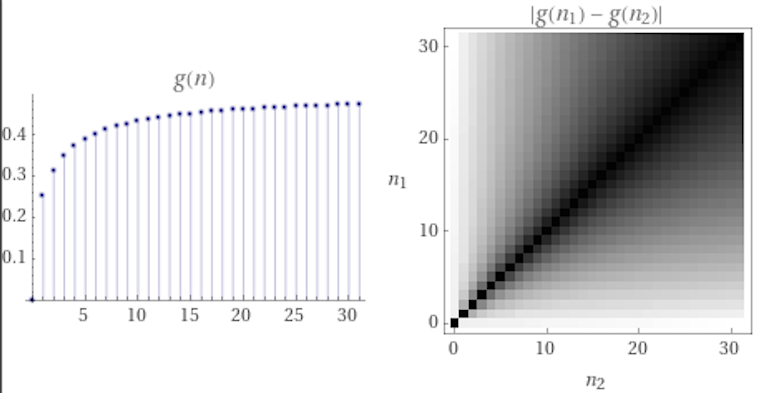
\includegraphics[scale=0.4]{Images/1.png}
\end{center}
\textbf{Con un $\alpha=0.1$, la convergencia es evidente.}
\begin{center}
    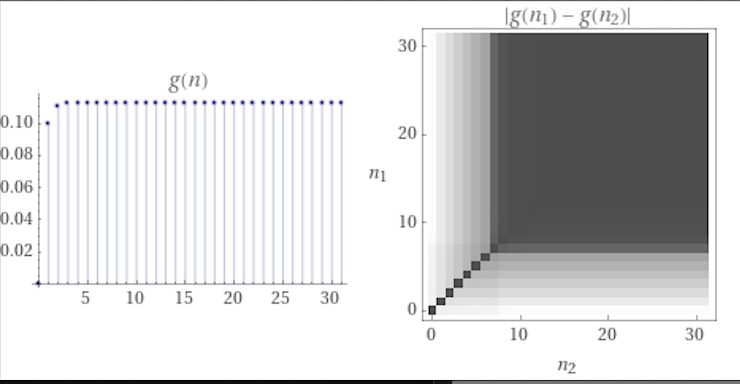
\includegraphics[scale=0.4]{Images/2.png}
\end{center}
\textbf{Con un $\alpha=0.5$, no existe convergencia.}
\begin{center}
    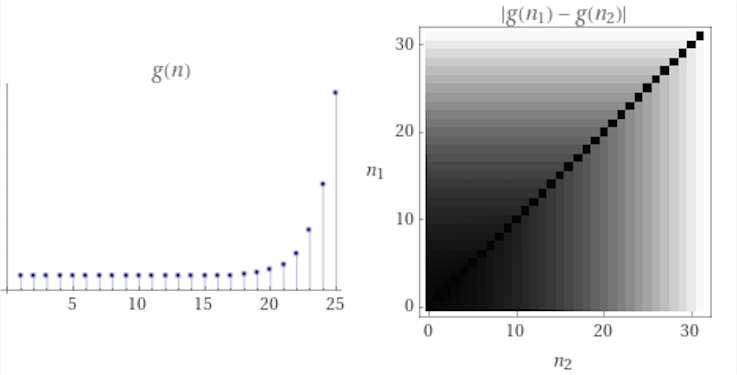
\includegraphics[scale=0.4]{Images/3.png}
\end{center}
Por lo tanto, la condición parece cumplirse.
%---------------------------
\bibliographystyle{apalike}
\bibliography{sample.bib}

\end{document}